\documentclass[11pt,a4paper]{article}

\usepackage{mathpazo}
\usepackage{microtype}
\usepackage{url}
\usepackage{verbatim}
\usepackage{graphicx}
\usepackage{float}

\usepackage{tikz}
\usetikzlibrary{external,positioning,through,calc,intersections}
\tikzexternalize[prefix=tikz/]

\textwidth=15cm
\textheight=23cm
\topmargin=18pt
\headheight=0pt
\oddsidemargin=2em
\headsep=0pt
\renewcommand{\baselinestretch}{1.1}
\setlength{\parskip}{0.3\baselineskip plus 1pt minus 1pt}
\parindent=0pt

\begin{document}
\thispagestyle{empty}

\begin{center}

\textbf{\huge Solving Motion and Work Problems}

\smallskip

\textbf{\huge with Graphs}


\bigskip
\bigskip
\bigskip

\textbf{\LARGE Moti Ben-Ari}

\bigskip

\textbf{\Large Department of Science Teaching}

\bigskip

\textbf{\Large Weizmann Institute of Science}

\bigskip

\url{http://www.weizmann.ac.il/sci-tea/benari/}

\end{center}

\bigskip
\bigskip

\begin{center}
\copyright{}\  2018 by Moti Ben-Ari.
\end{center}

This work is licensed under the Creative Commons Attribution-ShareAlike 3.0 Unported License. To view a copy of this license, visit \url{http://creativecommons.org/licenses/by-sa/3.0/} or send a letter to Creative Commons, 444 Castro Street, Suite 900, Mountain View, California, 94041, USA.

\bigskip
%
%%\begin{center}
%%
\includegraphics[width=.2\textwidth]{../by-sa.png}
%%\end{center}

\newpage

%\url{http://www.weizmann.ac.il/sci-tea/benari/mathematics/}.



%%%%%%%%%%%%%%%%%%%%%%%%%%%%%%%%%%%%%%%%%%%%%%%%%%%%%%%%%%%%%%%%

\newpage

\section*{a}

$A$,

$6$

$B$.

$A$,

$B$
$2$

$A$

$B$

$6$

\begin{center}
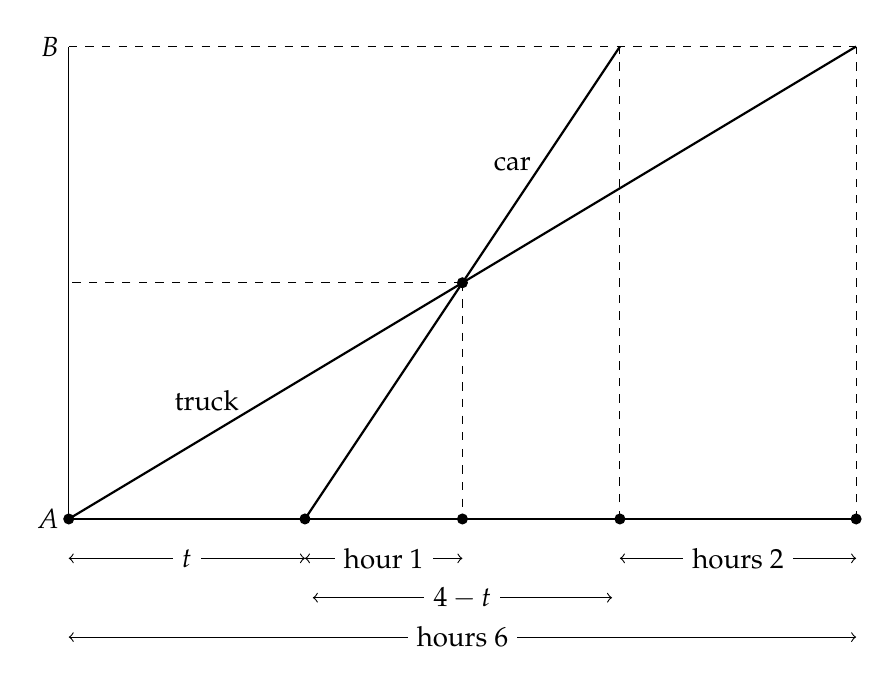
\begin{tikzpicture}
\draw (0,0) node[left] {$A$} -- (10,0);
\draw (0,0) -- (0,6) node[left] {$B$};
\draw[dashed] (0,6) -- (10,6);
\draw[thick,name path=truck] (0,0) -- node[left,near start,xshift=-6pt] {truck} (10,6);
\draw[thick,name path=car] (3,0) -- node[left,near end] {car} (7,6);
\path [name intersections={of=truck and car,by=meeting}];
\draw[dashed] (meeting) |- coordinate (time) (0,0);
\draw[dashed] (meeting) -| (0,0);
\draw[dashed] (10,0) -- (10,6);
\draw[dashed] (7,0) -- (7,6);
\fill (meeting) circle [radius=2pt];
\fill (time) circle [radius=2pt];
\fill (0,0) circle [radius=2pt];
\fill (3,0) circle [radius=2pt];
\fill (7,0) circle [radius=2pt];
\fill (10,0) circle [radius=2pt];
\draw[<->] (0,-.5) -- node[fill=white] {$t$} (3,-.5);
\draw[<->] (3,-.5) -- node[fill=white] {hour $1$} (time |- 0,-.5);
\draw[<->] (7,-.5) -- node[fill=white] {hours $2$} (10,-.5);
\draw[<->] (3.1,-1) -- node[fill=white] {$4-t$} (6.9,-1);
\draw[<->] (0,-1.5) -- node[fill=white] {hours $6$} (10,-1.5);
\end{tikzpicture}
\end{center}

$=t$
$=v_c$

$=v_m$


$A$
$A$

$B$:
\begin{eqnarray*}
v_m(t+1) &=& v_c\cdot 1\\
v_m \cdot 6 &=& v_c (4-t)\,.
\end{eqnarray*}

$t$:
\[
t^2 - 3t + 2 = 0
\]

$1=t$

$2=t$




%%%%%%%%%%%%%%%%%%%%%%%%%%%%%%%%%%%%%%%%%%%%%%%%%%%%%%%%%%%%%%%%


\newpage


\section*{b}


$10$

$2$

$\frac{1}{7}$





$3$


$3$


%%%%%%%%%%%%%%%%%%%%%%%%%%%%%%%%%%%%%%%%%%%%%%%%%%%%%%%%%%%%%%%%

\bigskip



\begin{center}
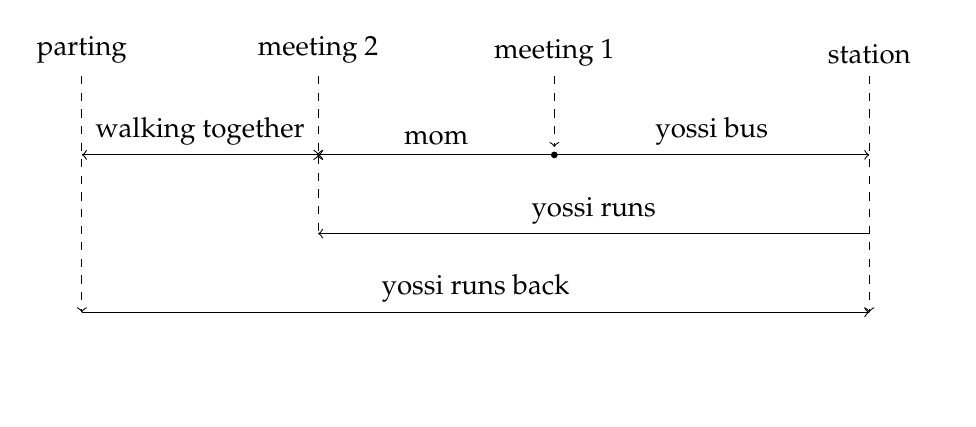
\begin{tikzpicture}
\draw[dashed,->] (4,1) node[yshift=1pt,above] {station} -- (4,-2);
\draw[dashed,->] (0,1) node[above] {meeting $1$} -- (0,.1);
\draw[dashed,->] (-3,1) node[yshift=1pt,above] {meeting $2$} -- (-3,0);
\draw[dashed,->] (-6,1) node[yshift=1pt,above] {parting} -- (-6,-2);
\draw[->] (0,0) -- node[above] {yossi bus} (4,0);
\draw[->] (0,0) -- node[above] {mom} (-3,0);
\draw[fill] (0,0) circle [radius=1pt];
\draw[->] (4,-1) -- node[above] {yossi runs} (-3,-1);
\path (0,-1) -- (0,-1.1);
\draw[->] (-3,0) -- node[above] {walking together} (-6,0);
\draw[<-,dashed] (-3,0) -- (-3,-1);
\draw[->] (-6,-2) -- node[above] {yossi runs back} (4,-2);
\path (0,-3.1) rectangle (5,.1);
\end{tikzpicture}
\end{center}


%%%%%%%%%%%%%%%%%%%%%%%%%%%%%%%%%%%%%%%%%%%%%%%%%%%%%%%%%%%%%%%%


\bigskip


\begin{center}
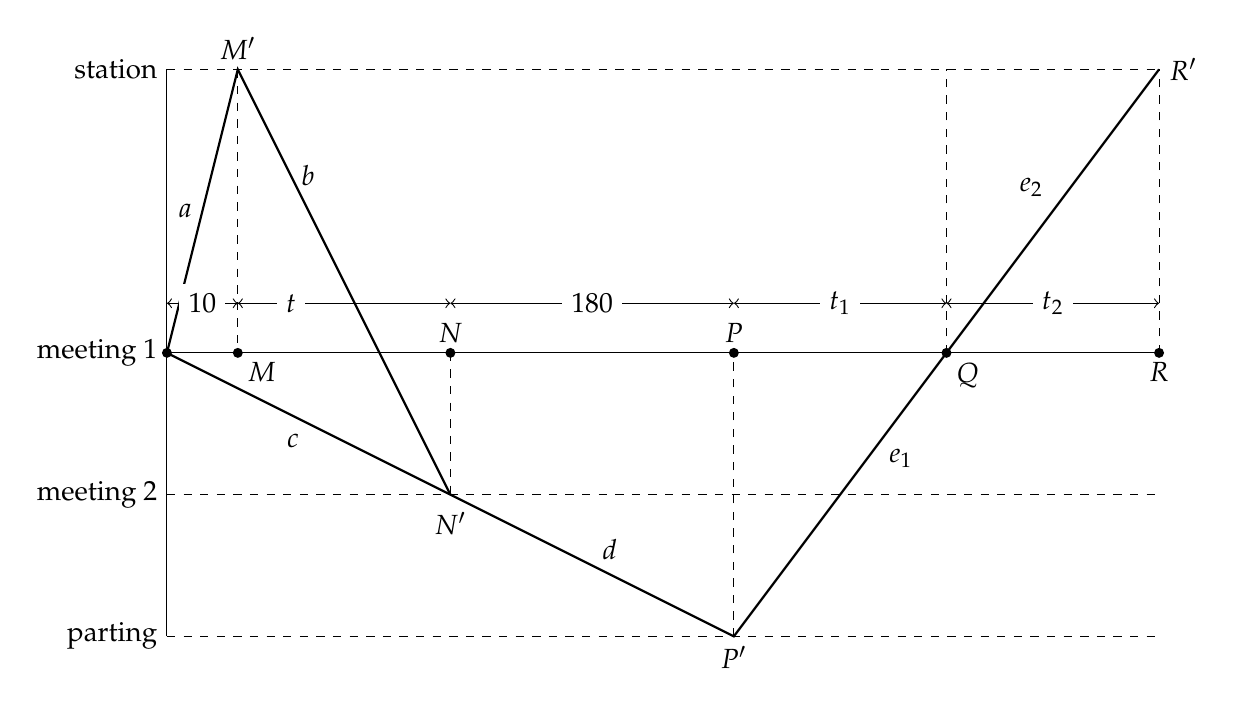
\begin{tikzpicture}[scale=.9]
\draw (0,0) -- (14,0);
\draw (0,-4) node[left] {parting} -- (0,-2) node[left] {meeting $2$} -- (0,0) node[left] {meeting 1} -- (0,4) node[left] {station};
\fill (0,0) circle [radius=2pt];
\fill (1,0) circle [radius=2pt] node[below right] {$M$};
\fill (4,0) circle [radius=2pt] node[above] {$N$};
\fill (8,0) circle [radius=2pt] node[above] {$P$};
\fill (11,0) circle [radius=2pt] node[below right] {$Q$};
\fill (14,0) circle [radius=2pt] node[below] {$R$};
\draw[thick] (0,0) -- node[left] {$a$} (1,4) -- node[right,near start] {$b$} (4,-2);
\draw[thick] (0,0) -- node[below,near start,xshift=-2mm] {$c$} node[right,near end,yshift=2mm] {$d$} (8,-4)  node[below] {$P'$} -- (14,4)  node[right] {$R'$};
\draw[dashed] (0,4) -- (14,4);
\draw[dashed] (0,-2) -- (14,-2);
\draw[dashed] (0,-4) -- (14,-4);
\draw[dashed] (1,4)  node[above] {$M'$} -- (1,0);
\draw[dashed] (4,0) -- (4,-2) node[below,yshift=-1mm] {$N'$};
\draw[dashed] (8,-4) -- (8,0);
\draw[dashed] (11,0) -- (11,4);
\draw[dashed] (14,0) -- (14,4);
\draw[<->] (0,.7) -- node[fill=white] {$10$} (1,.7);
\draw[<->] (1,.7) -- node[near start,fill=white] {$t$} (4,.7);
\draw[<->] (4,.7) -- node[fill=white] {$180$} (8,.7);
\draw[<->] (8,.7) -- node[fill=white] {$t_1$} (11,.7);
\draw[<->] (11,.7) -- node[fill=white] {$t_2$} (14,.7);
\path (8,-2) --  node[below right,xshift=5mm,yshift=-2mm] {$e_1$} (11,0);
\path (11,0) --  node[left,yshift=3mm] {$e_2$} (14,4);
\end{tikzpicture}
\end{center}


%%%%%%%%%%%%%%%%%%%%%%%%%%%%%%%%%%%%%%%%%%%%%%%%%%%%%%%%%%%%%%%%

$=a$

$=b$

$=c$

$=d$
$=e_1+e_2$




$=t$

$=v_y$

$=v_a$

$=v_b$


$v_y=2v_a$, $v_y=v_b/7$.

%%%%%%%%%%%%%%%%%%%%%%%%%%%%%%%%%%%%%%%%%%%%%%%%%%%%%%%%%%%%%%%%

\paragraph{a}

$NN'$
$1$

$2$.

$c$

$v_a(t+10)$.

$a$

$b$.

$NN'$.


\[
v_a(t+10) = v_yt - v_b \cdot 10.
\]

\[
\frac{v_y}{2}(t+10) = v_yt - 7\cdot v_y\cdot 10
\]

$150=t$

%%%%%%%%%%%%%%%%%%%%%%%%%%%%%%%%%%%%%%%%%%%%%%%%%%%%%%%%%%%%%%%%

\paragraph{n}


$e_1+e_2$


$PP'$

$1$

$e_1$,

$340=180+150+10$

$e_1$

$170=t_1$


$MM'$

$1$

$RR'=MM'$,

$e_2$,

$10$

$e_2$

$70=t_2$


$240=140+70=t_1+t_2$


$e_1$

$e_2$(,

$340=180+150+10$


%%%%%%%%%%%%%%%%%%%%%%%%%%%%%%%%%%%%%%%%%%%%%%%%%%%%%%%%%%%%%%%%

\section{c}



\section{ac}


\end{document}
